\documentclass[text06.tex]{subfiles}
\begin{document}
\newpage
\section{ヘッドセットの使い方}
\ruby{演習}{えん|しゅう}の前に、ヘッドセットの\ruby{設定}{せっ|てい}をしましょう。ヘッドセットとは、コンピュータなどから音声を出力するためのヘッドフォンと、コンピュータなどに音声を入力するためのマイクが一体型になったものです。

次の4つができれば、先へ進んでかまいません。マイクが使えなくなったときだけ、この節の最後の「\ruby{困}{こま}ったとき」を見てください。

\begin{enumerate}
\item \mbox{Raspberry Pi}の\ruby{電源}{でん|げん}を入れる前に、ヘッドセットをつないでおきます。
ヘッドセットが\mbox{Raspberry Pi}に\ruby{接続}{せつ|ぞく}されていると、画面の右上にマイクのアイコンが追加されます。

\begin{figure}[H]
\begin{center}
    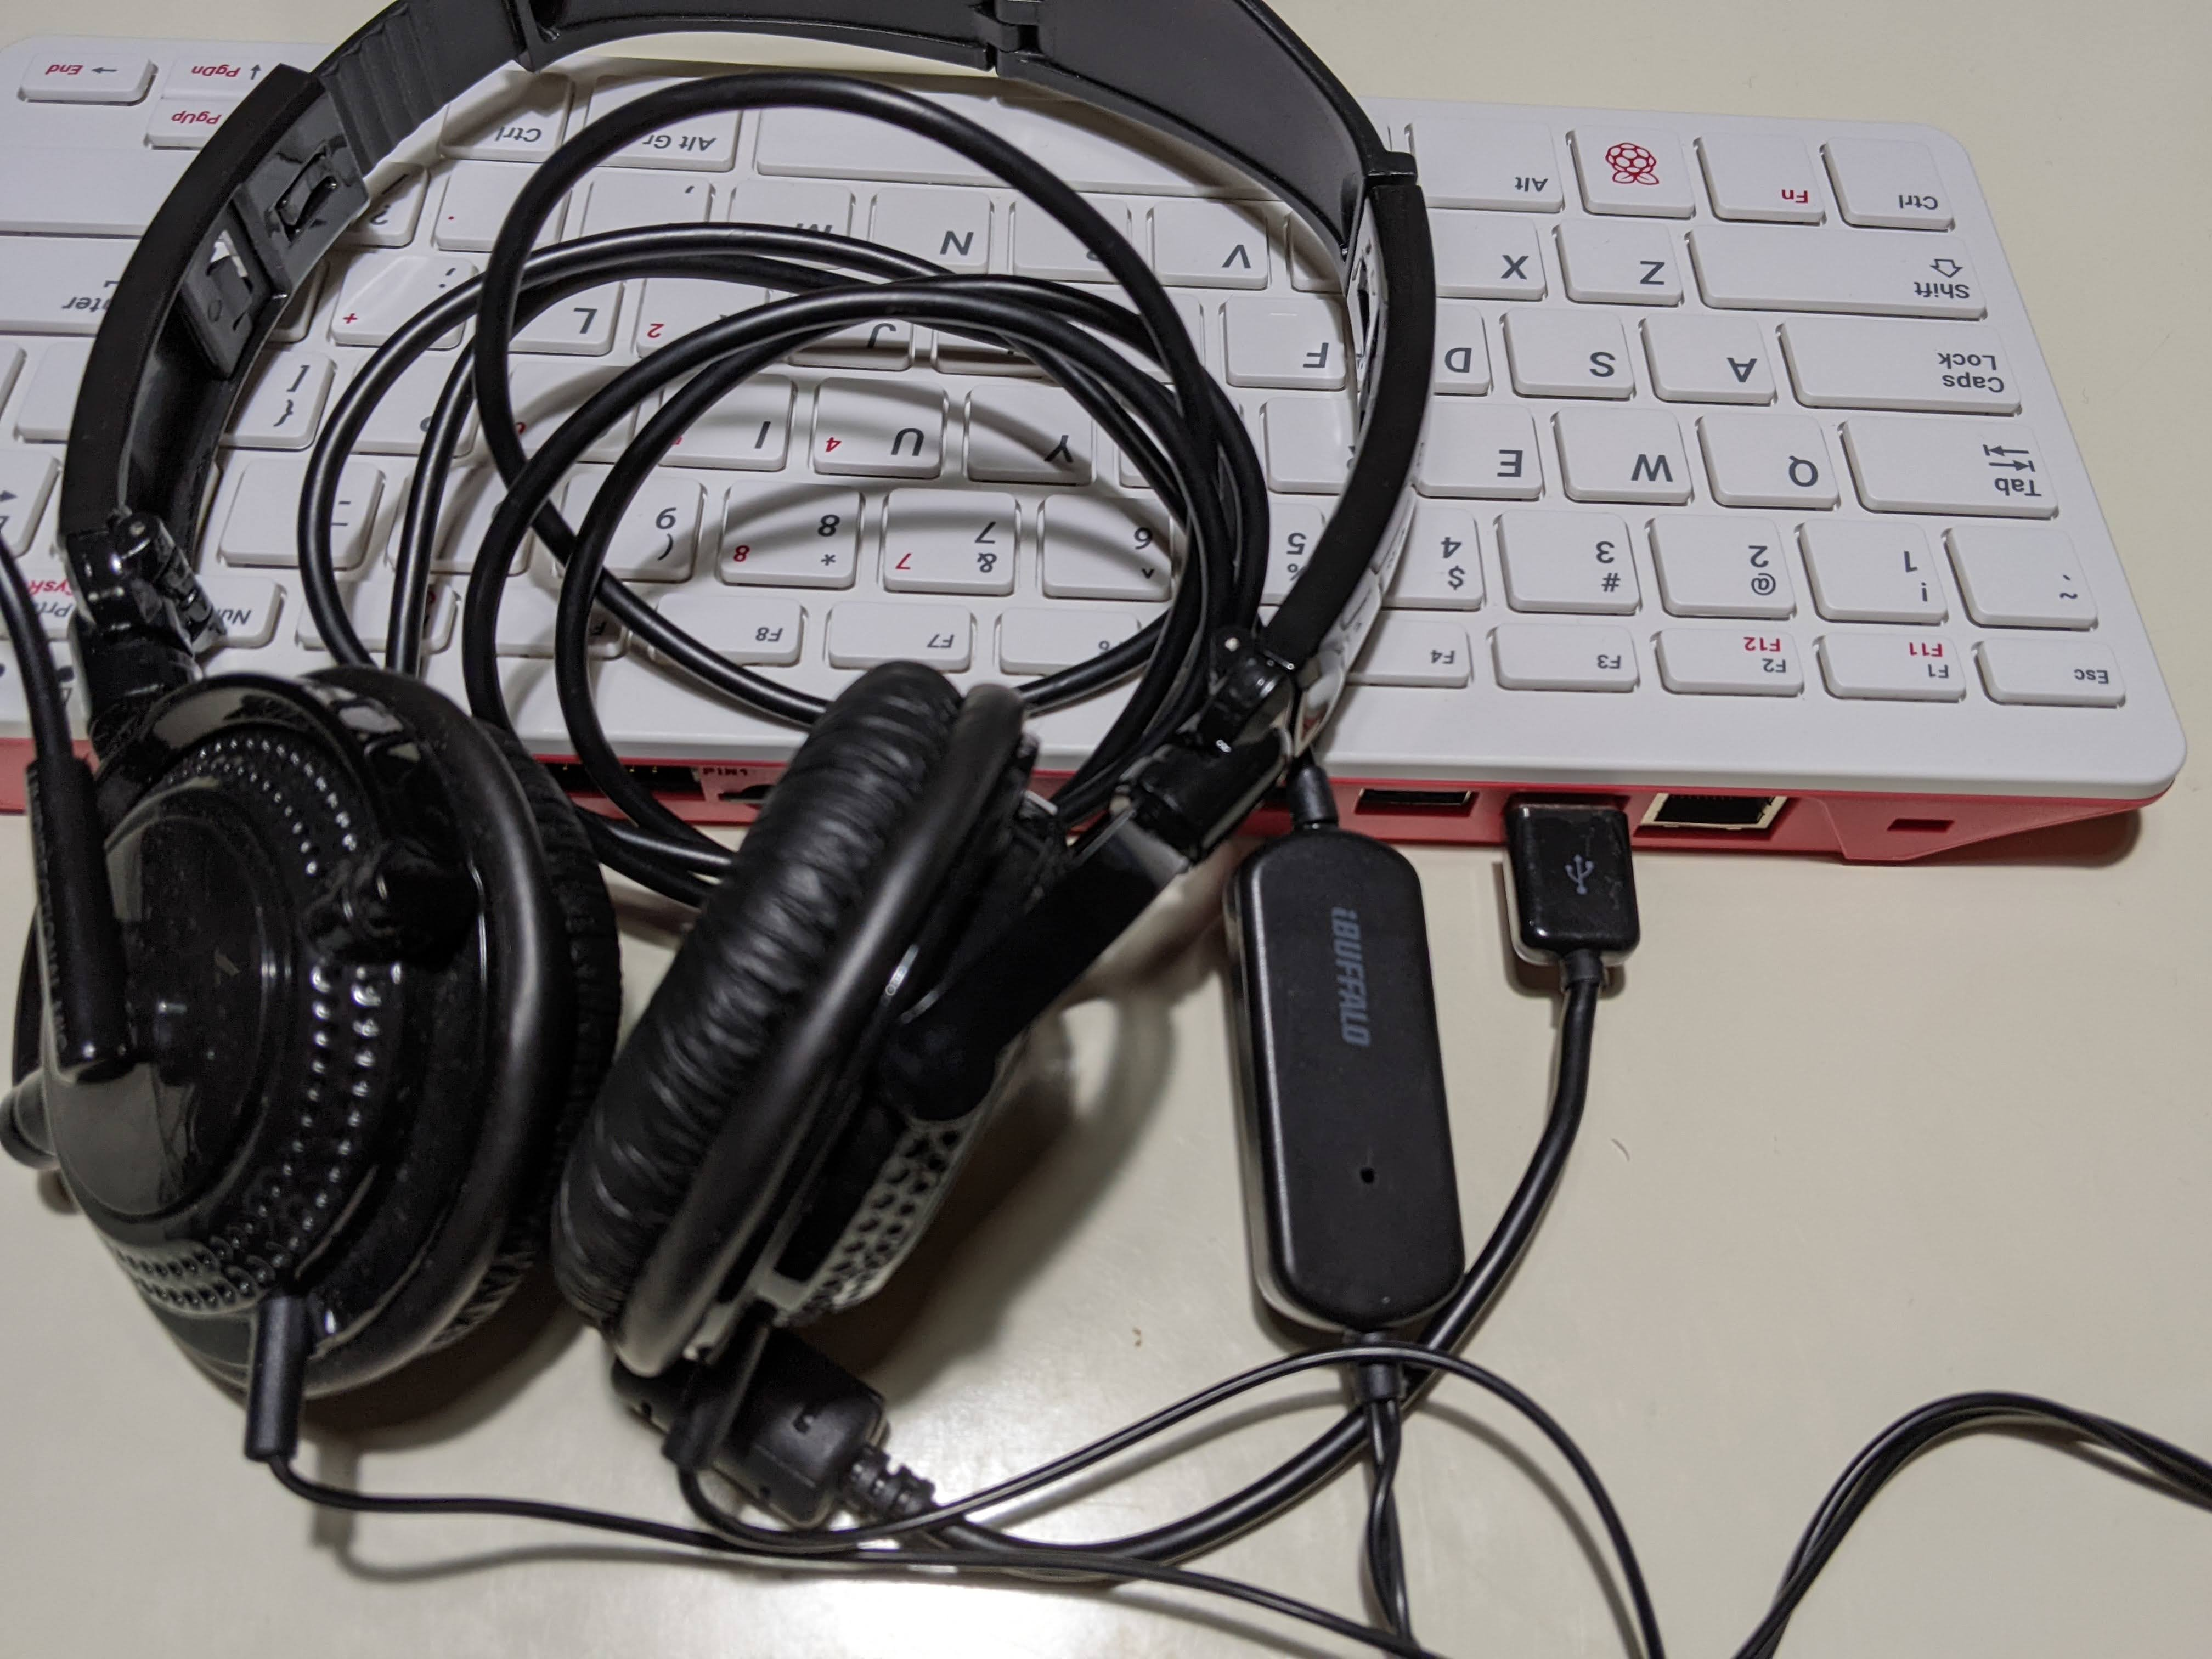
\includegraphics[width=.6\linewidth]{../../asset/image/how_to_connect_headset.jpg}
    \caption{ヘッドセットのつなげかた}
    \label{つなげかた}
\end{center}
\end{figure}

\item 音声出力として \aruby{USB}{ユーエスビー} \aruby{PnP}{プラグ・アンド・プレイ} \aruby{Sound}{サウンド} \aruby{Device}{デバイス} を\ruby{選択}{せん|たく}します。
ディスプレイの右上にあるスピーカーアイコンを右クリックしてください。図 \ref{使う音声デバイスの選択と設定} に使うことのできるデバイスが\ruby{表示}{ひょう|じ}されます。HDMIとはディスプレイのことです。教室ではヘッドセットを使うので、USB PnP Sound Device を左クリックします。おうちでは、ディスプレイやテレビから音声を出力することもできます。

\begin{figure}[H]
\begin{center}
    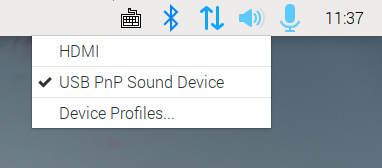
\includegraphics[width=.7\linewidth]{../../asset/image/select_sink.png}
    \caption{使う音声出力デバイスの選択と設定}
    \label{使う音声デバイスの選択と設定}
\end{center}
\end{figure}

\item マイクのミュートを\ruby{解除}{かい|じょ}します。
ヘッドセットのコントローラーの一番左のボタンで、マイクのミュートを切りかえることができます。ミュートとは音を消すことです。マイクがミュートしているときは赤色のLEDが光っています。マイクを使うときはミュートを解除して、赤色のLEDが光っていないようにしましょう。真ん中のボタンは音のミュートです。音が聞こえないときはここを\ruby{押}{お}してみましょう。右側のボタンは ``+" で音量を上げる、``-" で音量を下げることができます。

\begin{figure}[H]
\begin{center}
    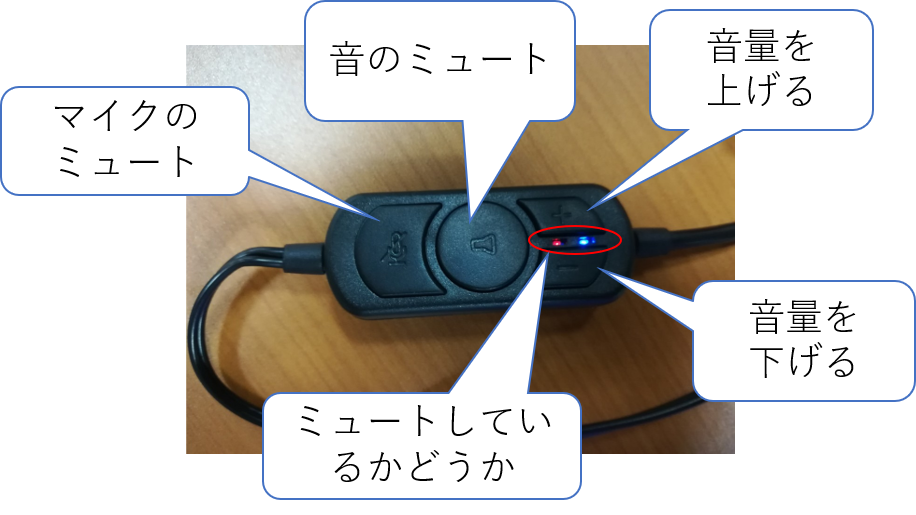
\includegraphics[width=.6\linewidth]{../../asset/image/text06-img004.png}
    \caption{ヘッドセットのコントローラーの使い方}
    \label{ヘッドセットのコントローラーの使い方}
\end{center}
\end{figure}

\item \ruby{必要}{ひつ|よう}なら、マイクの入力音量を\ruby{調節}{ちょう|せつ}します。
マイクのアイコンを左クリックし、表示されたスライドバーを調節します。教室では、図\ref{microphone_volume}のようにマイクの入力音量を最大にしておきましょう。

\begin{figure}[H]
\begin{center}
    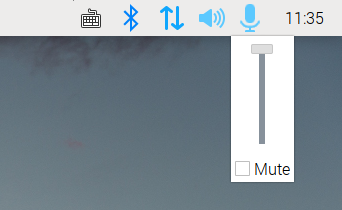
\includegraphics[width=.7\linewidth]{../../asset/image/microphone_volume.png}
    \caption{マイクの入力音量の調節方法}
    \label{microphone_volume}
\end{center}
\end{figure}
\end{enumerate}

設定ができたら、次の節に進みましょう。

\newpage
\subsection{\ruby{困}{こま}ったとき：マイクが使えなくなったら}
マイクのアイコンは、音量を変えるときだけ左クリックします。右クリックしたときに現れるメニューの「\aruby{USB}{ユーエスビー} \aruby{PnP}{プラグ・アンド・プレイ} \aruby{Sound}{サウンド} \aruby{Device}{デバイス}」（図 \ref{pplug-volume_mic_context_menu}）をクリックすると、一時的にマイクが使用できなくなります。図 \ref{pplug-volume_mic_context_menu} のように、チェックが外れている状態のときにマイクが使用できます。

\begin{itembox}[c]{\Large\textcolor{red}{注意！}}
マイクのアイコンを右クリックしたときに現れるメニューの「\aruby{USB}{ユーエスビー} \aruby{PnP}{プラグ・アンド・プレイ} \aruby{Sound}{サウンド} \aruby{Device}{デバイス}」はクリックしないように注意してください。
\end{itembox}

\begin{figure}[H]
    \begin{center}
      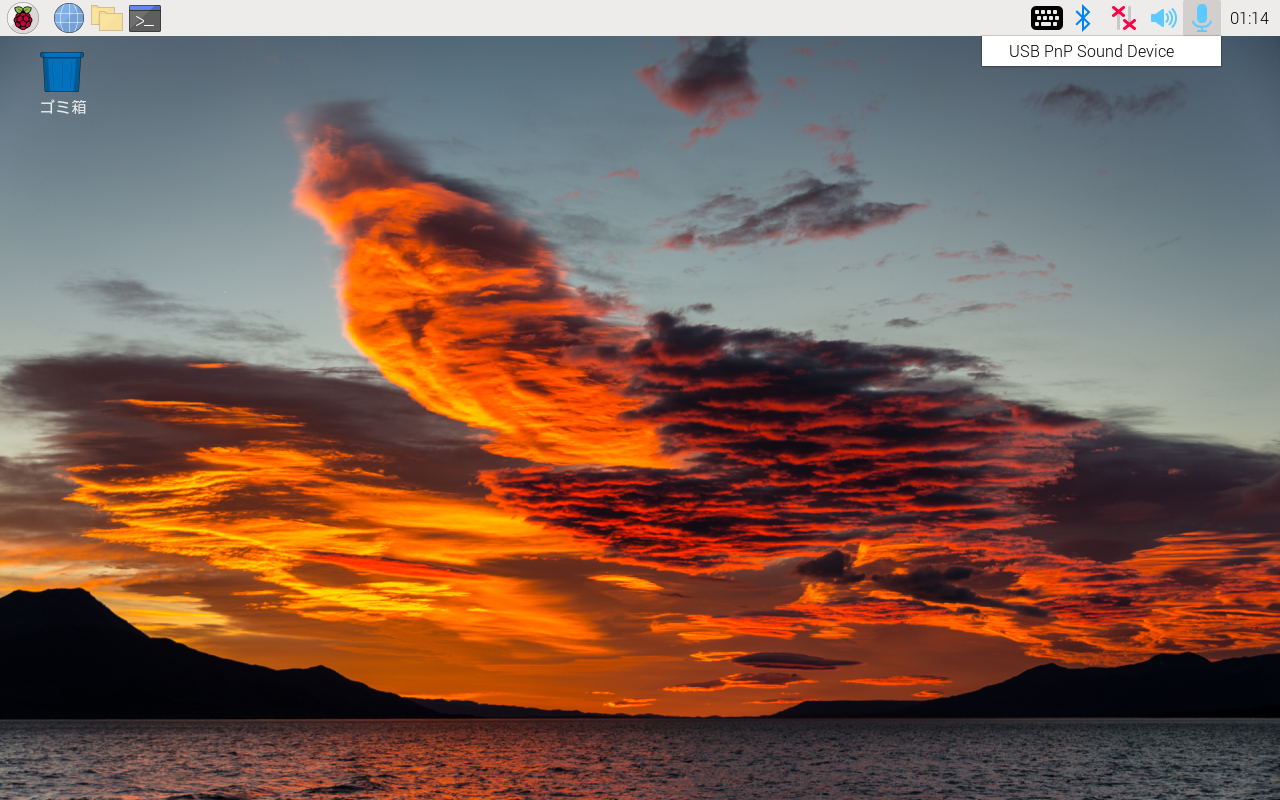
\includegraphics[width=\linewidth]{../../asset/image/pplug-volume_mic_context_menu.png}
      \caption{右上の USB PnP Sound Device はクリックしないよう注意！}
      \label{pplug-volume_mic_context_menu}
    \end{center}
\end{figure}

もしもマイクアイコンのメニューで「\aruby{USB}{ユーエスビー} \aruby{PnP}{プラグ・アンド・プレイ} \aruby{Sound}{サウンド} \aruby{Device}{デバイス}」を押してしまい、マイクが使えなくなってしまった場合は、以下の手順に従ってください。
まず、右上のスピーカーアイコンを右クリックし、「デバイスプロファイル…」をクリックしてください（図 \ref{pplug-volume_speaker_context_menu}）。
すると図 \ref{pplug-volume_device_profile_dialog_top} のように、新しいウィンドウが現れます。
USB PnP Sound Device の下にあるプルダウンメニューをクリックし、一度「アナログステレオ 出力」をクリックします（図 \ref{pplug-volume_device_profile_dialog_only_output}）。
もしはじめから「アナログステレオ 出力」が選択されていた場合は、一度「オフ」をクリックしてからもう一度「アナログステレオ 出力」をクリックしてください。
そのあと「アナログステレオ 出力 + モノ 入力」を選択してください（図 \ref{pplug-volume_device_profile_dialog_inout}）。
これで OK ボタンを押してデバイスプロファイルウィンドウを閉じれば、マイクが再度使えるようになっているはずです。

\begin{minipage}[ht]{0.23\linewidth}
    \begin{figure}[H]
        \begin{center}
            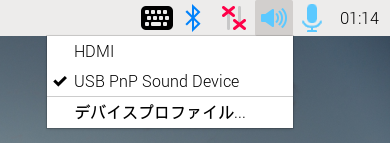
\includegraphics[width=\linewidth]{../../asset/image/pplug-volume_speaker_context_menu.png}
            \caption{USB PnP Sound Device にチェックを入れてしまったら、まずスピーカーアイコンを右クリック。}
            \label{pplug-volume_speaker_context_menu}
        \end{center}
    \end{figure}
\end{minipage}
\begin{minipage}[ht]{0.23\linewidth}
    \begin{figure}[H]
        \begin{center}
            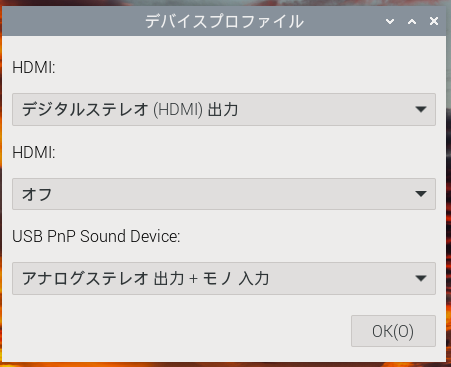
\includegraphics[width=\linewidth]{../../asset/image/pplug-volume_device_profile_top.png}
            \caption{「デバイスプロファイル」ウィンドウを表示}
            \label{pplug-volume_device_profile_dialog_top}
        \end{center}
    \end{figure}
\end{minipage}
\begin{minipage}[ht]{0.23\linewidth}
    \begin{figure}[H]
        \begin{center}
            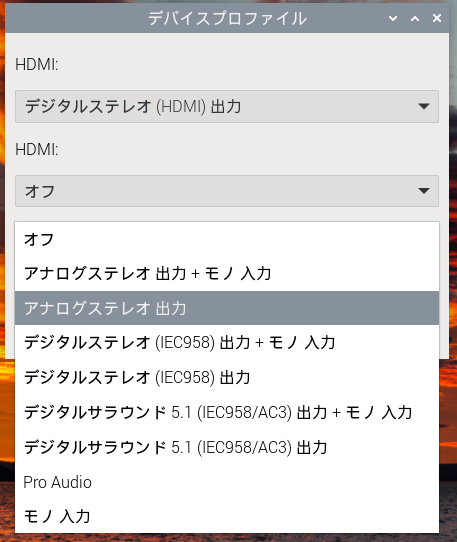
\includegraphics[width=\linewidth]{../../asset/image/pplug-volume_device_profile_dialog_only_output.png}
            \caption{一度「アナログステレオ 出力」を選択。}
            \label{pplug-volume_device_profile_dialog_only_output}
        \end{center}
    \end{figure}
\end{minipage}
\begin{minipage}[ht]{0.23\linewidth}
    \begin{figure}[H]
        \begin{center}
            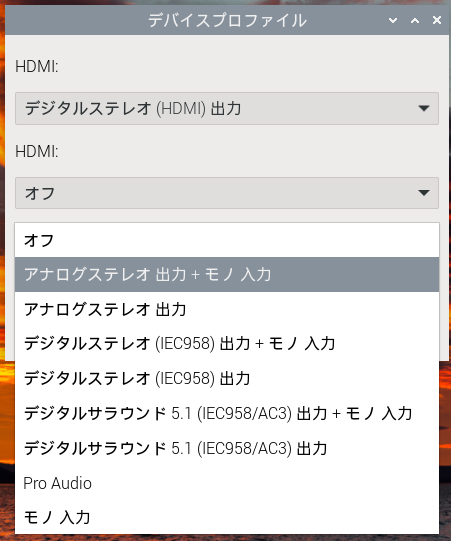
\includegraphics[width=\linewidth]{../../asset/image/pplug-volume_device_profile_dialog_inout.png}
            \caption{「アナログステレオ 出力 + モノ 入力」を選択し、「OK」。}
            \label{pplug-volume_device_profile_dialog_inout}
        \end{center}
    \end{figure}
\end{minipage}
\end{document}
